

\section{Surface visualization techniques}

In this section we will focus on different surface visualization techniques. Roughly we can divide surface mesh generation into \emph{model-based} and \emph{model-free}.

The model-based mesh generation makes some assumptions about the model, in our case about the vascular system.
In peculiar it makes assumptions about the topological structure, the observed junctions and the profiles of vessels. The topological structure is mostly represented by a graph and limited to a tree like representation. Also the observed junctions often are limited to certain kinds of junctions like bifurcations. Finally the profiles of the vessels are simplified to circular or elliptical structures.
All this simplifications and assumptions can help to speed up the process of surface generation, to make it more reliable or more visually pleasing or even transform the underlying data into more usable data for further processing. The downside is that model-based meshes do not resemble the underlying data as accurate as it could be done and also sometimes simplify the underlying data too much such that essential features are lost.
Especially when diagnoses of vascular degenerations or similar detail based inspections need to be done model-based approaches may not provide enough vivid information of the underlying data.

Here model-free mesh generation comes into play. The goal here is to retain as much of the underlying data as possible. But without a underlying model the extraction and creation of the mesh is more time consuming and cumbersome. Moreover unwanted results can arise if the underlying data suffers from noise or other failures in capturing. So care must be taken at the decision what for data is extracted and finally represented in the resulting mesh.

From the literature observed we determined that most of the methods require at some points a skeletonization of the underlying data. For now we assume that the underlying data consists of a voxel model that represents a density field of captured values. As model-based methods require a model, all of the observed methods require an extraction of a skeleton prior to the actual mesh generation. In regards of skeletonization the interested reader is reffered to Ebert et al.~\cite{ebert2002augmented} or  Strzodka et al.~\cite{strzodka2004generalized}.

As seen model-based mesh generation is based more or less on geometrical assumptions and reasoning on the model.
Volkau et al.~\cite{volkau2005geometric} for instance models a cerebral arterial model from segmented and skeletonized angiographic data. He constructs a vascular structure consisting of tube segments and bifurcations, so this model-based approach limits the domain of representable data quite hard in regards of branching possibilites. The centerline is smoothed with a sliding average filter to prevent problems with outliers and the two kinds of topologies, namely tubular and B-Subdivison based ones, are combined to form the complete vessel structure.

A connected graph is established that captures also the blood flow direction. This is done by splitting it up into two connected tree structures where one is designated as inflow structure. The model shapes the tube segments with decreasing radius with respect to the bloodflow as well as it captures radii change at bifurcations. This is based on statistical data. Radii at bifurcations are approximated with an exponential function whereas radii evolution at tubular parts are done via linear regression. At connection points C1 continuity is established via further constraints. So no abnormal cross section shape or diameter will show up easily in the final result.

\begin{figure}[h]
	\centering
	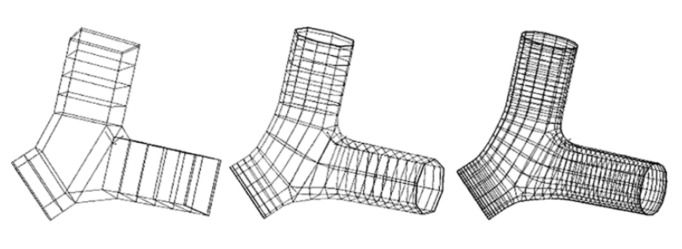
\includegraphics[width=0.4\textwidth]{./Images/B-subdivision_refinement.jpg} \\
	\caption{Example of refinement with B-subdivision.}
	\cite{volkau2005geometric}
	\label{fig:B-subdivision_refinement}
\end{figure}

The bifurcations themselves are constructed based on B-subdivison. The generation of quadrangles of a bifurcation till the overlapping internal part is shown in figure \ref{fig:B-subdivision_refinement}. Internal parts are subdivided to fit the outer subdivison. Problems with this scheme arise when all three vessels at the bifurcation form a close to orthogonal connection, where the inner face will be undefined. Also the B-subdivision of tubular segments show problems, namely self intersections when the radius of of curvature is smaller than the radius of the tube, shown in figure \ref{fig:Fold_of_vessel}.
Further problems mentioned are 'oversampling' or unrealistic sampling of bifurcations according to a too coarse sample pattern or problems with centerline smoothing in very jaggy areas as an acceptable smoothing also will remove esential features of the underlying vascular structure.  

\begin{figure}[h]
	\centering
	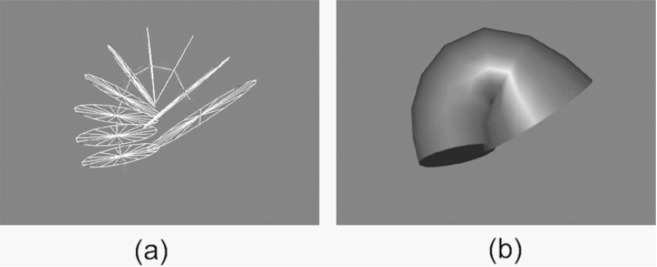
\includegraphics[width=0.4\textwidth]{./Images/Fold_of_vessel.jpg} \\
	\caption{Fold of vessel when curvature is higher than tube radius.}
	\cite{volkau2005geometric}
	\label{fig:Fold_of_vessel}
\end{figure}

\begin{figure}[h]
	\centering
	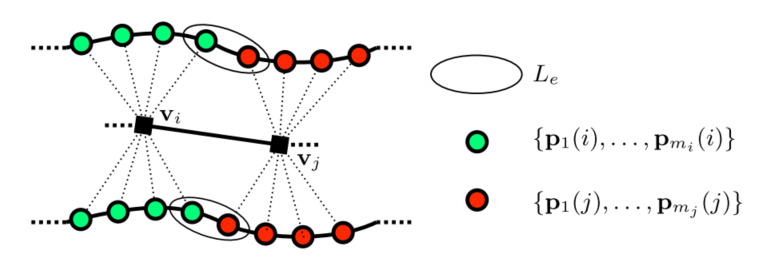
\includegraphics[width=0.4\textwidth]{./Images/Estimate_thickness.jpg} \\
	\caption{Estimation of thickness of graph edges.}
	\cite{sibbing2012topology}
	\label{fig:Estimate_thickness}
\end{figure}

Another geometry based modelling approach is provided by Sibbing et al.~\cite{sibbing2012topology}.
His work is focusing on quad meshes as they are visually more pleasant, require fewer elements and can produce more stable results in further processing, like FEM. Here the topologically correct extraction of the branching structure is done from a post-processed triangle mesh that is generated from an adapted \emph{Marching Cubes} algorithm based on the interior voxels which are identified via a variant of the \emph{Level Set} method. The extracted mesh is shrinked to a close to one dimensional structure that serves as basis for a tree based graph as well as for radius estimation along its edges, see figure \ref{fig:Estimate_thickness}. Further the graph is used to subdivide the triangle mesh into tubular parts and parts with one or more furcations with appropriate placed cutting planes. The so called \emph{interfaces} are 2D polygons between adjacent segments. They are defined by the intersection of cutting planes with the triangular mesh. 

Quad meshes for the junctions are created with the \emph{Mixed Integer Quadrangulation} by Bommes et al.~\cite{bommes2009mixed}. The quads are just required to align with the defined boundary to generate radially arranged quads.

\begin{figure}[h]
	\centering
	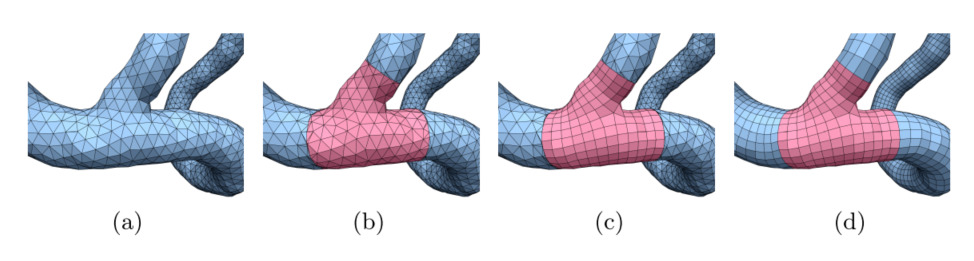
\includegraphics[width=0.45\textwidth]{./Images/Remeshing_stage.jpg} \\
	\caption{ (a) The input to our remeshing stage is a smoothed and resampled version of the mesh extracted using the Marching Cubes Algorithm. (b) The mesh is partitioned into junction and tube components. The cuts insert additional vertices at the respective interfaces. (c) We remesh the junctions yielding a fair quad layout. (d) Tubes are remeshed, such that the final mesh is a quad dominant mesh.}
	\cite{sibbing2012topology}
	\label{fig:Remeshing_stage}
\end{figure}

Tubes now only have to provide a smooth transition between two interfaces with a possibly different number of vertices. The rings of the tubes are generated out of equidistant iso-contours on the harmonic scalar field on the tube. Triangles are introduced between so called transition rings to compensate for the difference in vertices. The distribution of the transition rings as well as the distribution of the triangles around the tube in a transition case is done via adaption of the Bresenham line rasterization algorithm. Stretching of quads along the tube axis as well as rotations of the rings to get configurations with almost $90$ degree angles in the quads, yields close to optimal quad dominant meshes. The advantage of this reconstruction is the smoothing of unwanted artifacts on the original triangle mesh as well as the already shown properties of quad meshes, see figure \ref{fig:Remeshing_stage}.

%Describe skeletonization, e.g Topology aware Quad Dominant Meshing p.4f

\begin{figure}[h]
	\centering
	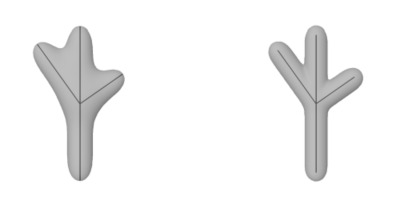
\includegraphics[width=0.33\textwidth]{./Images/Branching_ConvolutionSurfaces.jpg} \\
	\caption{Transition at branching.}
	\cite{oeltze2005visualization}
	\label{fig:Branching_ConvolutionSurfaces}
\end{figure}

A technique that uses the vessel skeleton as input data but only respects the diameter information at the provided graph is called \emph{convolution surfaces}. The main idea is that \emph{implicit surfaces} describe the original surface by equations to model smooth, deformable objects. Oeltze et al.~\cite{oeltze2005visualization} used a combination of so called 'blobs' to model an \emph{iso-surface} out of this scalar field function.
The resulting convolution surface is a surface of an object around its skeleton. The convolution itself is done on an integral of 'blob-functions' along the skeleton. It is actually the modification of a signal by a filter, in this case a Gaussian filter. To speed up the process filter functions with finite support are used and the scalar field is only computed within certain bounding volumes around the line segments. Unwanted blending at branchings is avoided by more narrow filter kernels, see figure \ref{fig:Branching_ConvolutionSurfaces}. Blending between segments that are close but not connected is avoided by restricted support on the skeleton, see figure \ref{fig:Blending_ConvolutionSurfaces}.

\begin{figure}[h]
	\centering
	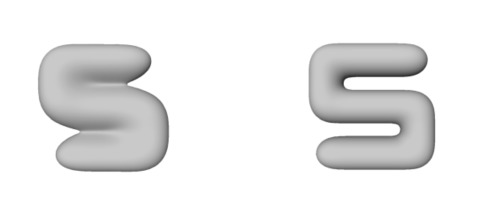
\includegraphics[width=0.33\textwidth]{./Images/Blending_ConvolutionSurfaces.jpg} \\
	\caption{Unwanted blending.}
	\cite{oeltze2005visualization}
	\label{fig:Blending_ConvolutionSurfaces}
\end{figure}

Still the problems of convolution surfaces are that they only support a circular base shape at tubes, that unwanted bulging can be suppressed but not completely removed and that unwanted blending of close parts is still possible. Finally the end segments have always the shape of a half sphere which neither represents the normally open ends of vascular trees nor has low deviation from the original surface in that areas.

In contrast model-free mesh generation mostly rely on some implicit functions that should resemble the input data instead of explicit constructive reasoning in geometric elements like tubes and junctions. Also here there are different techniques that respect the original shape more or less. Convolution surfaces therefore form a bridge between model-based and model-free mesh generation as the technique already use an implicit function but limit the shape in a model-based fashion.

\begin{figure}[h]
	\centering
	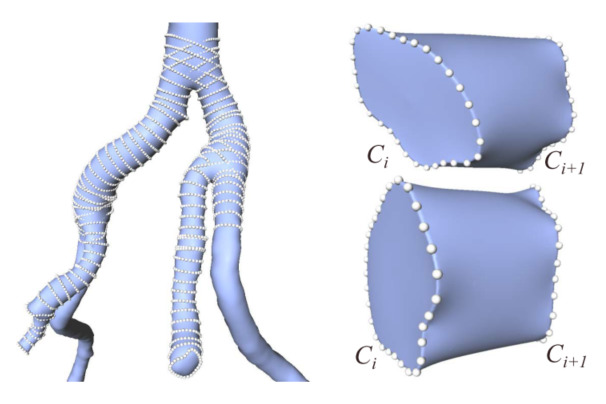
\includegraphics[width=0.33\textwidth]{./Images/ReconstructionFreeFormContours.jpg} \\
	\caption{Reconstruction of an arterial tree from free-form contours.}
	\cite{kretschmer2012reliable}
	\label{fig:ReconstructionFreeFormContours}
\end{figure} 

\begin{figure}[h]
	\centering
	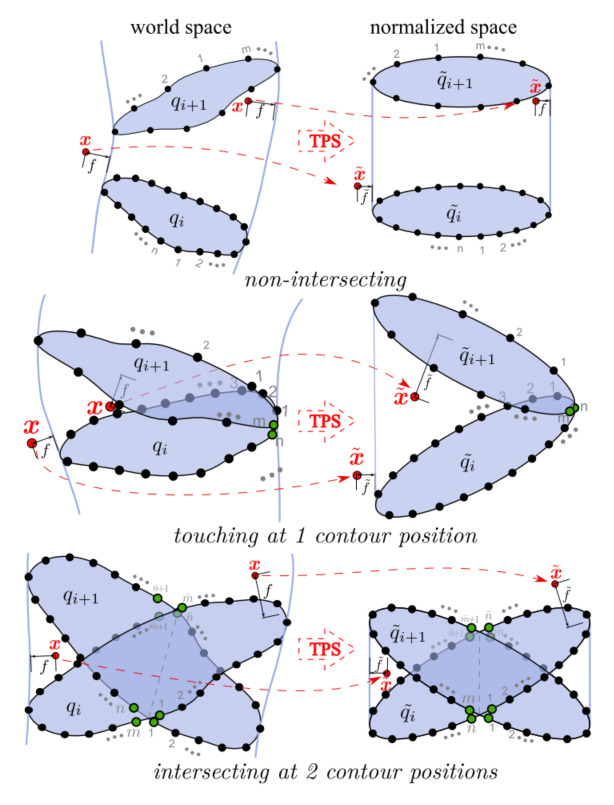
\includegraphics[width=0.33\textwidth]{./Images/IntersectingContours.jpg} \\
	\caption{Mapping of neighboring free-form contour pairs to normalized shapes.}
	\cite{kretschmer2012reliable}
	\label{fig:IntersectingContours}
\end{figure} 

To capture vascular profiles and open endings of vascular structures Kretschmer et al.~\cite{kretschmer2012reliable} uses an adaptive modelling with non circular cross sections. He generates intersection-free surfaces from centerlines with complex outlines, see fituge \ref{fig:ReconstructionFreeFormContours}. He decomposes the centerline description into segments which are locally described by implicit functions and combines them using boolean operations. In this fashion all intersection- and furcation-related issues are solved in similar fashion to convolution surfaces with the difference that the capturing of the vascular outline is not so limited. A watertight scale-adaptive mesh is generated out of an adaptive octree in the end. The key difference to CS is that the so called \emph{admissible distance functions} (ADFs) just form a class of functions with the property to detect valid iso-surfaces. To find a topology-preserving mapping that forms a intersection free surface part between two adjacent contours on the vascular structure found by the ADFs they follow the idea of \emph{thin plate splines}. The assignment of contour pairs to a limited set of target shapes guarantee a valid surface topology when the contours do not touch, touch or penetrate each other as shown in figure \ref{fig:IntersectingContours}.

\begin{figure}[h]
	\centering
	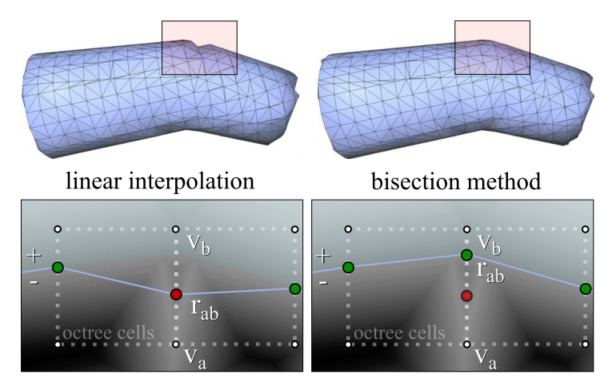
\includegraphics[width=0.4\textwidth]{./Images/BisectionMethod.jpg} \\
	\caption{Improved root-finding of the iso-surface using bisection method.}
	\cite{kretschmer2012reliable}
	\label{fig:BisectionMethod}
\end{figure} 

The octree that should capture also the smallest vessels is recursivly subdivided at surface intersections with the grid. To speed up queries on the octree a localized approximation of the implicit function with a certain threshold to safely prune cells is used.
To improve the quality of the extracted mesh a bisection method is used to interpolate between values when marching cubes is applied, advantages of this scheme is shown in figure \ref{fig:BisectionMethod}.

\begin{figure}[h]
	\centering
	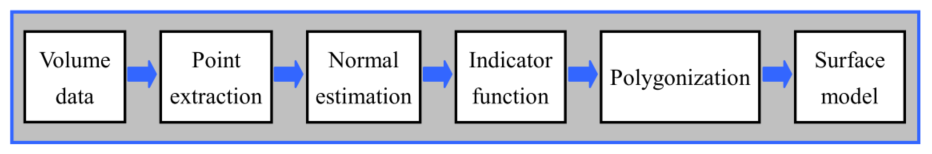
\includegraphics[width=0.45\textwidth]{./Images/Pipeline.png} \\
	\caption{Pipeline of geometric modeling of vascular tree structures.}
	\cite{wu2010scale}
	\label{fig:Pipeline}
\end{figure} 

Finally Wu et al.~\cite{wu2010scale} also generates scale-adaptive surfaces from vascular structures with similar properties. He extracts the vascular boundary voxels from the segmentation and use them to build a 3D point cloud where normals are estimated via covariance analysis. Then a 3D implicit indicator function os computed from the point cloud ba solving a Poisson equation. Finally the surface is generated by adaptive polygonization.
The surface is a smooth, morphologically topology correct two-manifold that is scale-apdaptive to the local curvature ans have fewer and better shaped triangles compared to earlier approaches. The pipeline used is shown in figure \ref{fig:Pipeline}. 

To reconstruct very thin vessel structures an adaptive point extraction is used that relies on the constellation of adjacent object voxels. Normals are estimated on k-nearest neighbours of a point in the point cloud and the smallest eigenvalue of their covariance matrix. The implicit function that approximates the surface of the point samples is a Poisson surface reconstruction. It utilize the vector field and generates a function gradient best approximates the normal field of the point cloud.

\begin{figure}[h]
	\centering
	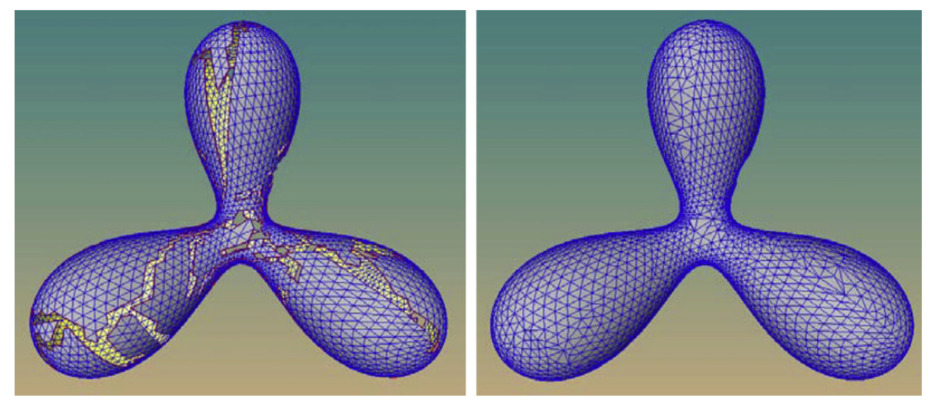
\includegraphics[width=0.4\textwidth]{./Images/Polygonization.jpg} \\
	\caption{Polygonization of a trifurcate model. A long gap is produced upon the termination of mesh
		expanding stage (left), and is sewed in the subsequent gap-stitching stage (right).}
	\cite{wu2010scale}
	\label{fig:Polygonization}
\end{figure} 

\begin{figure}[h]
	\centering
	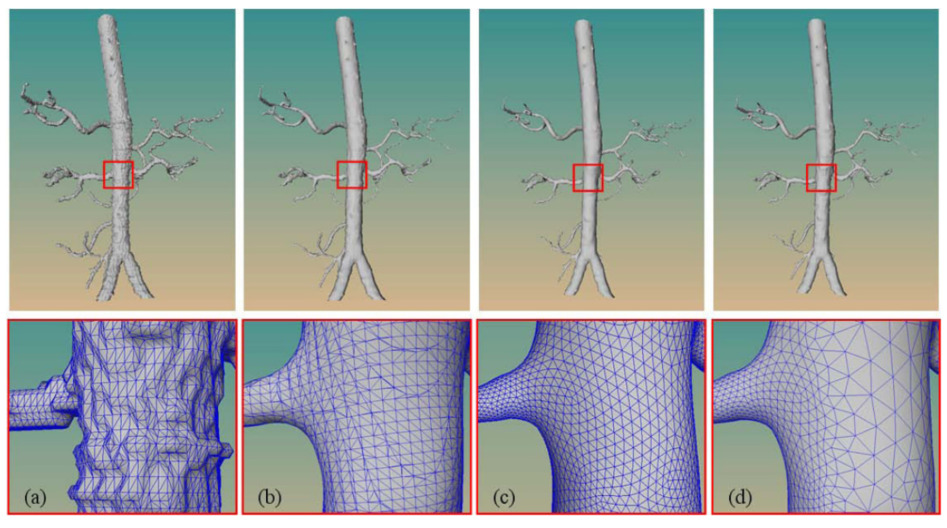
\includegraphics[width=0.4\textwidth]{./Images/TriangleQuality.jpg} \\
	\caption{ Comparison of triangle quality for an aorta tree. Surface model generated by the marching cubes (a),
		multi-level partition unity based method (b), subdivison surface based method (c) and sclae-adaptive surface method (d). The bottom row is a zoomed region corresponding to the rectangle region of the top row.}
	\cite{wu2010scale}
	\label{fig:TriangleQuality}
\end{figure} 

The polygonization is done by an advancing front algorithm utilizing Newton step method. Care has been taken to ensure that the minimal angle of triangles is maximized in the triangulation step. The resulting gap on the surface is then closed via a stitching operation, see figure \ref{fig:Polygonization}. Also here the patching triangles are subdivided to a similar size than the surrounding ones. To further refine and smooth the mesh a Loop based subdivison is performed.
A comparison of several methods is shown in figure \ref{fig:TriangleQuality}. It can be seen that the scale-adaptive nature of the reconstructed mesh together with the smooth and but still good approximation of the underlying shape yields very good results on vascular structures. 
